\section{Interference Analysis}
\label{sec:interference}

\textbf{\emph{Intra-job interference}} refers to the network contention between ranks within each application. \textbf{\emph{Inter-job interference}} is introduced by concurrently running jobs that adjacent to each other sharing network resources. Communication variability due to such interference can cause application performance degradation.

In this section we will study both kinds of interference in the context of torus network. 
Since application's communication pattern won't change with its scale, we use AMG with 216 ranks, CrystalRouter with 100 ranks, and MultiGrid 125 ranks. And in order to accommodate three applications running concurrently with different allocations, we simulate a 2K-node 3D torus ($16^{2} \times 8$) network for the experiments.


\subsection{Intra-Job Interference Analysis}
\label{sec: introjob}

We design two sets of experiments to study the intra-job interference of each application. In the first, shown in Figure \ref{fig:shapestudy}, we assign each application with allocations in \emph{three different shapes}.  In the second, shown in Figure \ref{fig:diffmap}, we study the intra-job interference by using different mapping strategies for each application with given allocation shape. 

In the allocation shapes experiment, we select three possible shapes can can commonly seen on the 3D torus network. They are 3D balanced-cube, 3D unbalanced-cube, 2D mesh, as shown in Figure \ref{fig:alloc-shapes}.

3D balanced-cube, shown as red in Figure \ref{fig:cont_sub1}, can guarantee the minimum \emph{average pair-wise distance} within the allocation. Some research studies like \cite{leung,abhinav-sc13} indicate that compact allocation can guarantee jobs with better performance. They use a variety of metrics to evaluate the compactness of the allocation, such as \emph{average pair-wise distance}, \emph{diameter} and \emph{contiguity}. In this work, we select 3D balanced-cube as the most compact allocation on a 3D torus network.

3D unbalanced-cube, shown as green in Figure \ref{fig:cont_sub1}, is a rectangular prism, which is the possible allocation shape on the systems with asymmetric networks. For example, Cray XE6/XK7 systems are deployed 3D tori with Gemini routers. The network connections in the \emph{y}-direction have only half the bandwidth of the cables used in the \emph{x} and \emph{z} directions. In order to take advantage of the faster links in the \emph{x} and \emph{z} directions, job allocation starts from X-Z plane, which leads to a rectangular prism shaped allocation \cite{RF}.

2D mesh, shown as blue in Figure \ref{fig:cont_sub1}, can be cut out from a single layer of the 3D torus. 2D mesh is a very common allocation shape in torus network for both contiguous and non-contiguous allocation strategies. For example, Cray Application Level Placement Scheduler (ALPS) indexes the nodes in torus network into a list and makes job allocation by simply going through the list \cite{carl-cug}. When the list is obtained by sorting the nodes based on their spacial coordinates in the torus, allocation made off from this list will be 2D mesh. The IBM Blue/Gene Q supercomputer Mira at Argonne Leadership Computing Facility also allow its allocation partition configured into mesh \cite{zhou-ipdps}. 

\begin{figure*}[t!]
    \centering
    \begin{subfigure}[t]{0.2\textwidth}
        \centering
        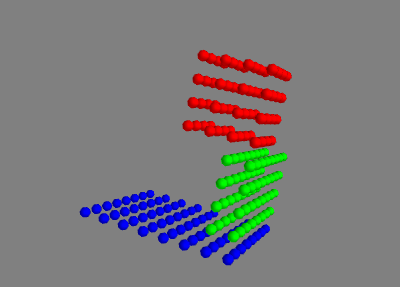
\includegraphics[height=1.2in]{figs/allocshape/allocation}
        \caption{ }
        \label{fig:cont_sub1}
    \end{subfigure}%
    \hspace{1em}%
    \begin{subfigure}[t]{0.2\textwidth}
        \centering
        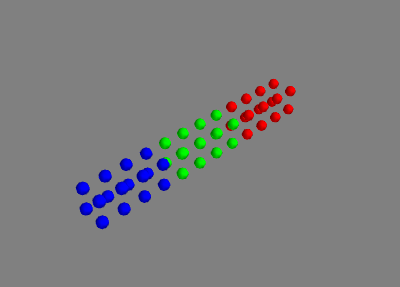
\includegraphics[height=1.2in]{figs/allocshape/unitsize/unit16}
        \caption{ }
        \label{fig:noncont_sub1}
    \end{subfigure}%
    \begin{subfigure}[t]{0.2\textwidth}
        \centering
        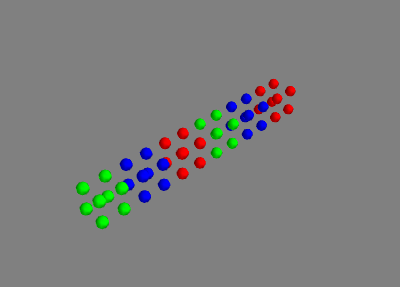
\includegraphics[height=1.2in]{figs/allocshape/unitsize/unit8}
        \caption{ }
        \label{fig:noncont_sub2}
    \end{subfigure}%
    \begin{subfigure}[t]{0.2\textwidth}
        \centering
        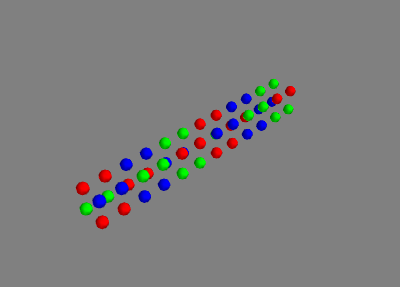
\includegraphics[height=1.2in]{figs/allocshape/unitsize/unit2}
        \caption{ }
        \label{fig:noncont_sub3}
    \end{subfigure}%
    \caption{(a) Contiguous allocation in three different shapes. ``Blue" is 2D mesh, ``Green" is 3D-unbalanced cube and ``Red" is 3D-balanced cube. (b)-(d) Non-contiguous allocation. Each job is represented by a specific color. The nodes assigned to different jobs are interleaved, the size of allocation unit are 16, 8 and 2.}
    \label{fig:alloc-shapes}
\end{figure*}


AMG with 3D ``Nearest Neighbor" communication pattern takes less time when being assigned with 3D-unbalanced allocation than 3D-balanced, as shown in Figure \ref{fig:shapstudy-amg}. And MultiGrid gets the best performance (shortest data transfer time) when running on 3D-balanced allocation, as shown in Figure \ref{fig:shapstudy-mg}. Since MultiGrid's communication pattern is ``Many-to-Many" dominant, 3D-balanced is the most compact allocation with shortest pair-wise distance between nodes, which can reduce the aggregated hops for transferring message among ranks in MultiGrid. As CrystalRouter has both dominant local communication and multi-stage global data transfer, the 3D-balance is also the best allocation, but its advantage over 3D-unbalanced is not that obvious as to MultiGrid, as shown in Figure \ref{fig:shapstudy-cr}.

Lots of research studies have designed complex allocation algorithms to provide application with the most compact allocation\cite{leung,LO}. However, as shown in our experiments, providing cubical allocation without considering application's communication pattern can not guarantee the best performance for every application. Compact allocation should be provided to application with global data transfer, such as those conforms to ``Many-to-Many" communication pattern. Application with dominant communication pattern like ``Nearest Neighbor" won't fully utilize the compact allocation and could get even better performance on a relaxed allocation shape. 



\begin{figure*}[t!]
    \centering
    \begin{subfigure}[t]{0.32\textwidth}
        \centering
        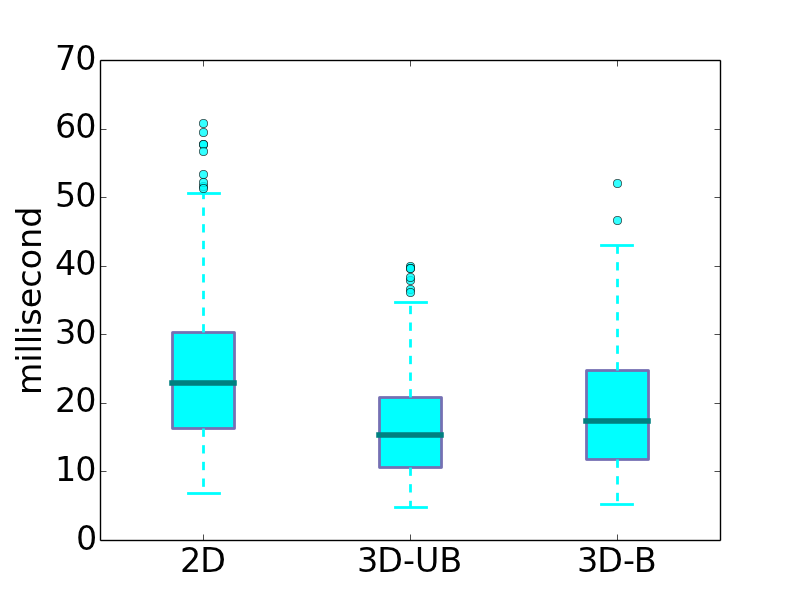
\includegraphics[height=1.5in]{figs/intra-job/shapestudy/amg_box}
        \caption{AMG}
        \label{fig:shapstudy-amg}
    \end{subfigure}%
    \hspace{1em}%
    \begin{subfigure}[t]{0.32\textwidth}
        \centering
        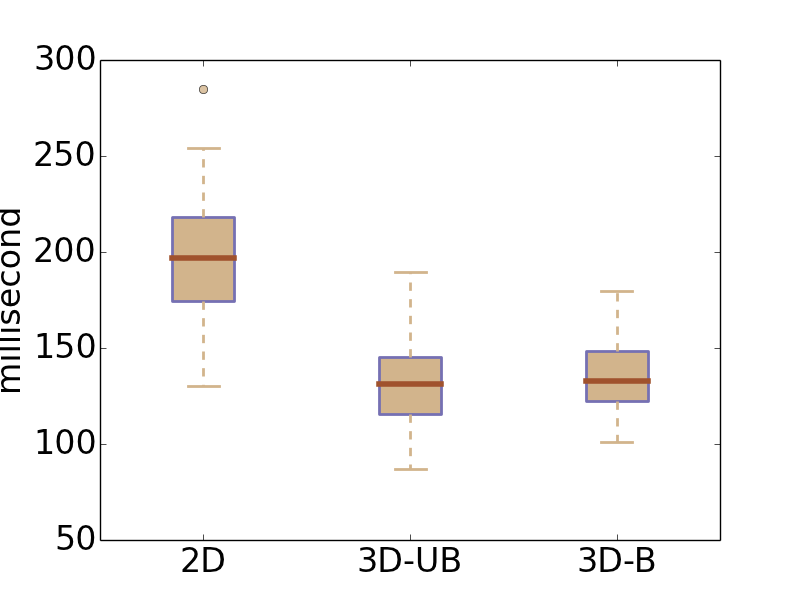
\includegraphics[height=1.5in]{figs/intra-job/shapestudy/cr_box}
        \caption{CrystalRouter}
        \label{fig:shapstudy-cr}
    \end{subfigure}%
    \begin{subfigure}[t]{0.32\textwidth}
        \centering
        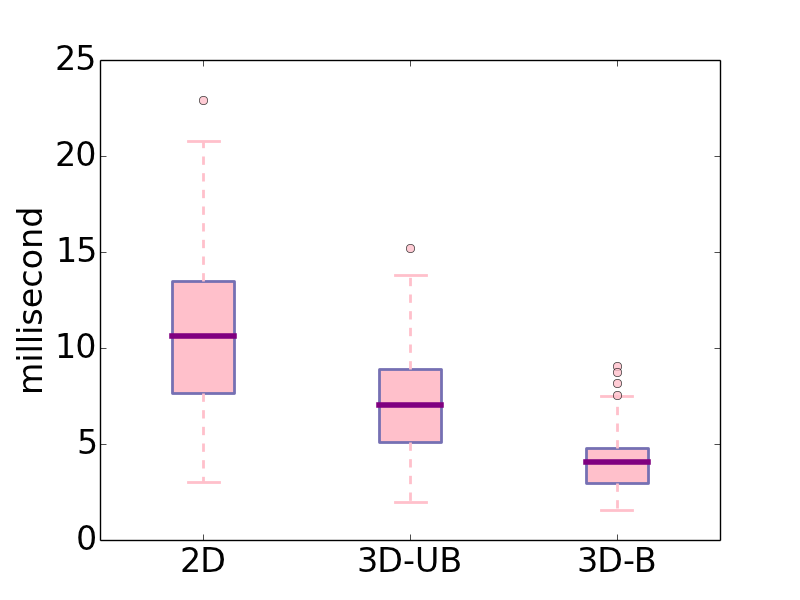
\includegraphics[height=1.5in]{figs/intra-job/shapestudy/mg_box}
        \caption{MultiGrid}
        \label{fig:shapstudy-mg}
    \end{subfigure}%
   \caption{Data transfer time of AMG, CrystalRouter and MultiGrid on 3D-balanced, 3D-unbalanced and 2D allocation.}
   \label{fig:shapestudy}
\end{figure*}


The rank-to-node mapping of parallel applications on HPC system could greatly impact applications' performance. However, finding the optimal mapping solution for a given application is out the scope of this work. Our experiments aims to show how mapping strategies impact the intra-job interference of application with specific communication pattern.

We provide AMG, CrystalRouter and MultiGrid with 3D-balance allocation and use three mapping strategies to do the rank-to-node mapping. The ``Linear" mapping, as we used in the previous experiments, is to map each rank according to the dimensional ordering of compute nodes. The ``Cube" mapping assigns ranks into consecutive $2^{3}$ cubes. The ``Random" mapping assigns ranks randomly within the allocation. 

AMG remains roughly the same when it been mapped by ``Linear" and ``Cube", shown in Figure \ref{fig:diffmap-amg}. Although ``Linear" and ``Cube" mapping strategies cause some routing overlap for AMG's communication, both mapping strategies still preserve the locality of AMG's 3D ``Nearest Neighbor" communication pattern. The ``Random" mapping totally destroys AMG's communication pattern, and results in intra-job interference among all the ranks in AMG. The performance degradation caused by using ``Random" mapping is up to 90\%.

The ``Cube" mapping improves CrystalRouter's performance over the ``Linear" by reducing the pair-wise distance between ranks, shown in Figure \ref{fig:diffmap-cr}. The global data transfer in CrystalRouter will takes fewer hops with ``Cube" mapping. The ``Random" mapping scatters the ranks within the local neighborhood of CrystalRouter and make their communication less efficient. 


The ``Cube" mapping benefits MultiGrid's ``Many-to-Many" communication. However, due to the small amount of data transfer among ranks in MultiGrid, ``Cube" mapping fails to exhibit a drastic advantage. ``Random" mapping neither cause too much degradation for the same reason, shown in Figure \ref{fig:diffmap-mg}.


\begin{figure*}[t!]
    \centering
    \begin{subfigure}[t]{0.32\textwidth}
        \centering
        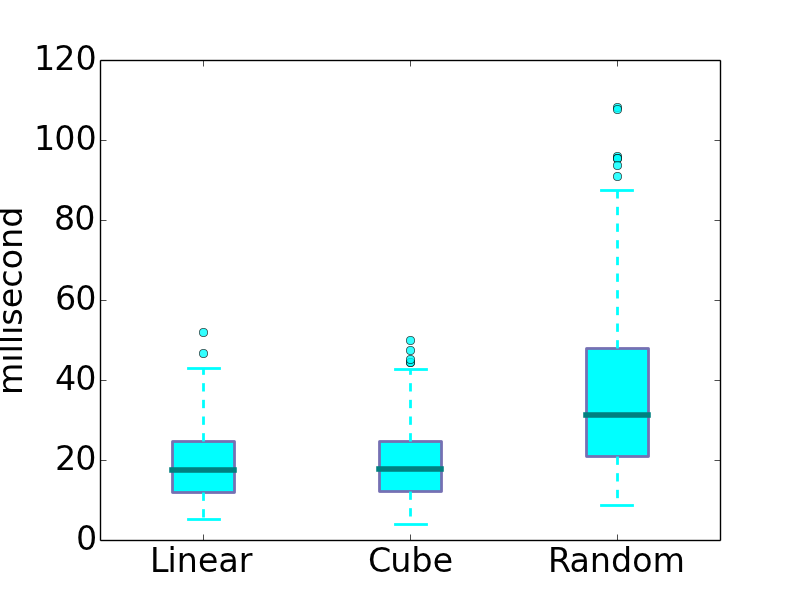
\includegraphics[height=1.5in]{figs/diffmapping/amg}
        \caption{AMG}
        \label{fig:diffmap-amg}
    \end{subfigure}%
    \hspace{1em}%
    \begin{subfigure}[t]{0.32\textwidth}
        \centering
        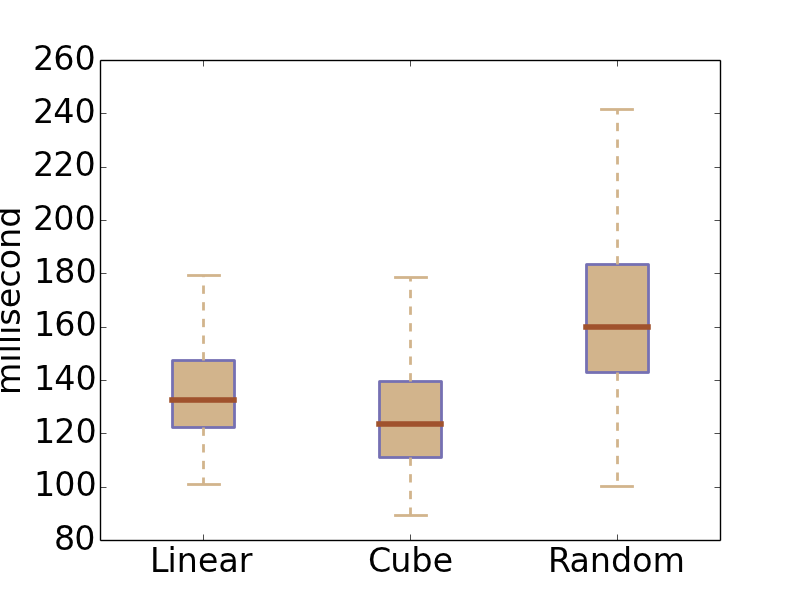
\includegraphics[height=1.5in]{figs/diffmapping/cr}
        \caption{CrystalRouter}
        \label{fig:diffmap-cr}
    \end{subfigure}%
    \begin{subfigure}[t]{0.32\textwidth}
        \centering
        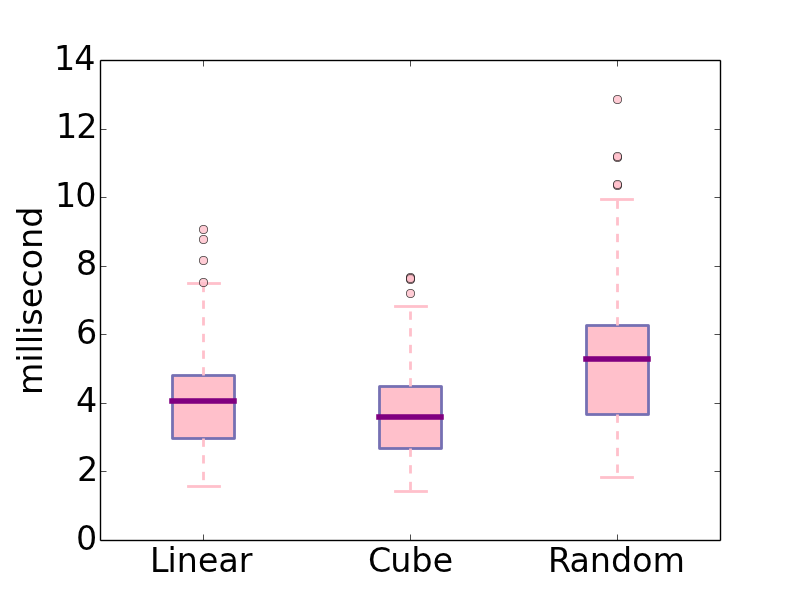
\includegraphics[height=1.5in]{figs/diffmapping/mg}
        \caption{MultiGrid}
        \label{fig:diffmap-mg}
    \end{subfigure}%
   \caption{Data transfer time of AMG, CrystalRouter and MultiGrid on 3D-balanced allocation using  different mapping strategies.}
   \label{fig:diffmap}
\end{figure*}




\subsection{Inter-Job Interference Analysis}
\label{sec: interjob interference study}

Inter-job interference has been identified as one of the major culprits for application's performance variability \cite{abhinav-sc13,skinner,rosenthal}. Inter-job interference is a more prominent issue for system adopted non-contiguous allocation policy than system with contiguous allocation. Application communication times have been demonstrated to vary from 36\% faster to 69\% slower due to job interference when running on non-contiguous allocation \cite{abhinav-sc13}.

We assign each application with non-contiguous allocation and run them concurrently on the same network. The allocation unit belongs to different jobs are interleaved. In order to study the impact of different allocation unit size on applications' inter-job interference, we conduct experiments with unit size of 16, 8 and 2, shown respectively in Figure \ref{fig:noncont_sub1}, \ref{fig:noncont_sub1} and \ref{fig:noncont_sub3}. Figure \ref{fig:interjobstudy} shows the results of each application data transfer time with different allocation unit size. 

The data transfer time of AMG in Figure \ref{fig:interjob-amg} keeps stable between allocation unit size of 16 and 8, since the locality of AMG is 6-rank based. When the unit size reduce to 2, AMG suffers prolong data transfer time by about 10\%. CrystalRouter is more sensitive to allocation unit size. The best unit size would be the one big enough to accommodate its local neighborhood. Figure \ref{fig:interjob-cr} shows unit size of 16 and 8 can guarantee the same average data transfer time, while some rank spend more time with allocation unit size 8 than 16. When the unit size reduce to 2, the communication become less efficiency and takes about 15\% more times for transferring data. 

The data transfer time of MultiGrid with different allocation unit sizes doesn't show obvious variability in Figure \ref{fig:interjob-mg}. This is because even big allocation unit size like 16 will still fail to preserve MultiGrid's ``Many-to-Many" pattern. The data transfer time is almost doubled when MultiGrid running concurrently with allocation unit size of 16, as shown in Figure \ref{fig:interjob-mg} . As the unit size decreases, the data transfer time keep growing, but in a slow way, which means in terms of preserving the locality of MultiGrid, allocation unit of size 16, 8 and 2 serve equally bad.

The unit size in non-contiguous allocation policy should be chosen according to application's communication pattern. Inter-job interference is inevitable in non-contiguous based systems, but unit size that big enough to preserve the neighborhood communication of the application will alleviate such interference and improve job performance. 



\begin{figure*}[t!]
    \centering
    \begin{subfigure}[t]{0.32\textwidth}
        \centering
        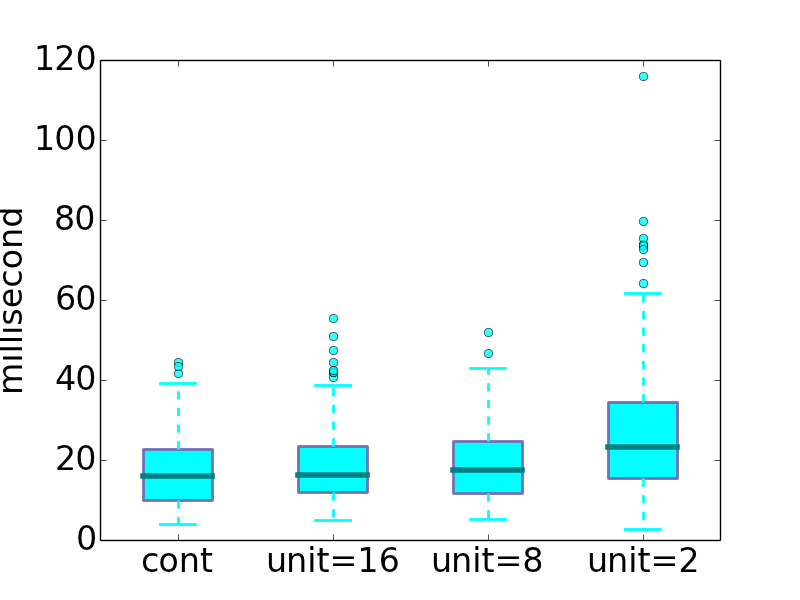
\includegraphics[height=1.5in]{figs/inter-job/amg}
        \caption{AMG}
        \label{fig:interjob-amg}
    \end{subfigure}%
    \hspace{1em}%
    \begin{subfigure}[t]{0.32\textwidth}
        \centering
        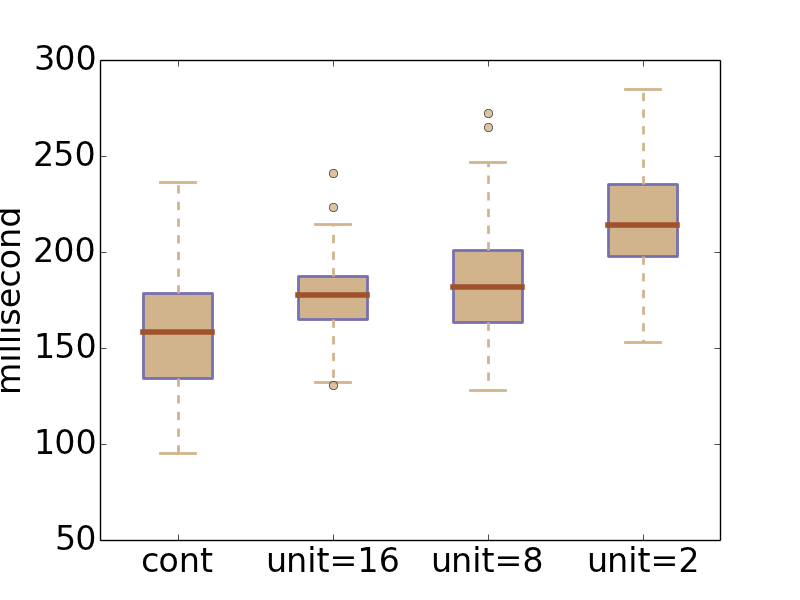
\includegraphics[height=1.5in]{figs/inter-job/cr}
        \caption{CrystalRouter}
        \label{fig:interjob-cr}
    \end{subfigure}%
    \begin{subfigure}[t]{0.32\textwidth}
        \centering
        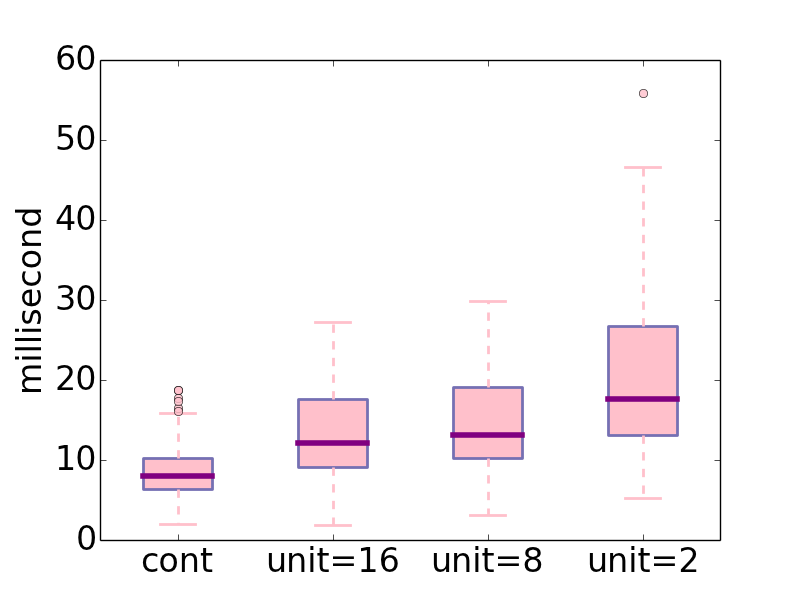
\includegraphics[height=1.5in]{figs/inter-job/mg}
        \caption{MultiGrid}
        \label{fig:interjob-mg}
    \end{subfigure}%
   \caption{Inter-job interference study. ``cont" indicates three applications running side by side concurrently on the same network with contiguous allocation. To study the impact of non-contiguous allocation on inter-job interference, applications running concurrently with interleaved allocation of different unit sizes, which are 16-node, 8-node, 2-node. }
   \label{fig:interjobstudy}
\end{figure*}

\subsection{Result Summary}
\label{sec:summary}

Based on the above comprehensive study, we can make following observations:
\begin{itemize}
    \item The compact allocation may not guarantee the best performance for every application. 
    \item The applications dominated with Nearest Neighbor communications exhibit relatively stable performance under different allocation shapes, while the applications dominated with Many-to-Many communication exhibit better performance with compact allocation (e.g. 3D balanced).
    \item A good rank-to-node mapping strategy can greatly improve application's performance when specific allocation is given.
    \item An optimal size for allocation units should be determined according to an application's dominant communication pattern. In general, a unit size should be large enough to preserve neighboring communication of the application. 
    \item Inter-job interference is inevitable in non-contiguous allocation. However, choosing the proper allocation unit size with job's communication pattern awareness can alleviate such negative effect. 
\end{itemize}





